\chapter{Réalisation}\label{realisation}


\section{Capture d'image}\label{realisation.capture}
\subsection{Emplacement de la caméra}
En date du 29 mai 2018, la caméra a été installée, connectée au réseau et est fonctionnelle. La photo présentée en figure \ref{fig:cam_parking_annotation} est une vue aérienne du site de Cheseaux de la HEIG-VD. C'est ici qu'un parking sera filmé.

\begin{figure}[H]
    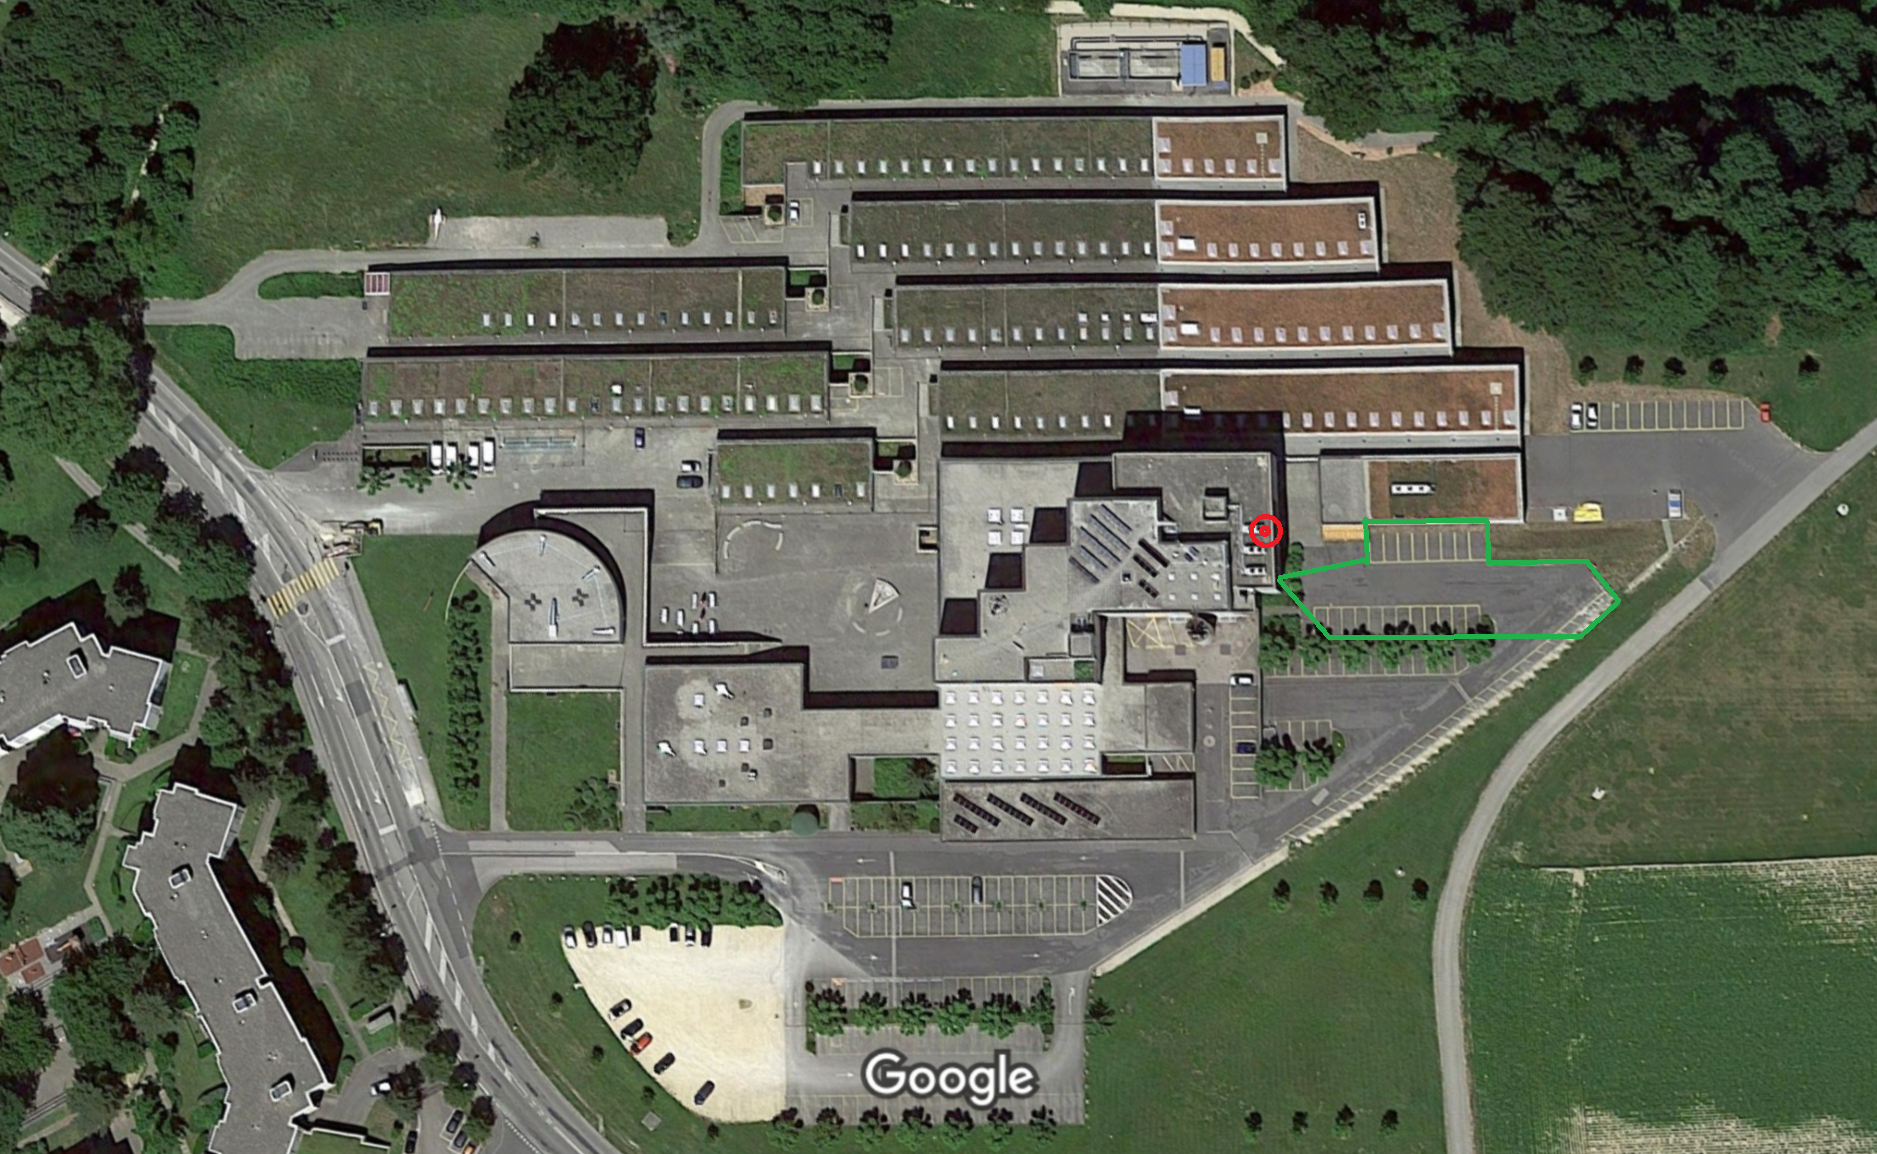
\includegraphics[width=130mm]{img/conception/cam_parking_location.png}
    \label{fig:cam_parking_annotation}
    \centering
    \captionsource{Emplacement de la caméra (en rouge) et du parking filmé (en vert)}{map:heig-vd}
\end{figure} 

Y est désigné par un cercle rouge l'emplacement de la caméra. Elle se situe sur la terrasse du bâtiment est, accessible au niveau K. Elle est orientée afin de pouvoir capturer des images du parking désigné en vert. 

Malheureusement, lors des tests effectués après réception de la caméra \textbf{Wanscam} \textit{HW0029-5}, il a été remarqué que le signal Wifi présent sur le toît n'était pas suffisamment fiable afin de connecter la caméra. Afin de palier à ce problème, un câble réseau Ethernet a été tiré de manière temporaire.

\subsection{Configuration des périphériques}
Dans cette sous-section, on trouvera des informations utiles concernant la caméra et la machine virtuelle. Ces informations seront utilisées dans la suite de ce rapport. 

Afin de pouvoir accéder à la caméra, un FQDN\footnote{\textit{FQDN}: \textit{Fully qualified domain name}, soit nom de domaine entièrement qualifié. \autocite{wiki:FQDN}} a été configuré. Celui-ci permet d'obtenir l'adresse IP de la caméra à l'aide du DNS local. Ainsi, plutôt que de s'adresser à une adresse IP, il suffit d'utiliser en lieu et place l'adresse suivante:
\begin{center}
    \textit{ipcam.einet.ad.eivd.ch}
\end{center}

%\nomenclature{FQDN}{\textit{Fully qualified domain name}, soit nom de domaine entièrement qualifié}

Comme indiqué en section \ref{conception.architecture.capture.logique}, une VM est mise à disposition de ce projet afin de récupérer des images de la caméra. Son adresse IP, 10.192.75.100, est fixe.

\subsection{Requêtes et protocole}
La caméra \textbf{Wanscam} \textit{HW0029-5} expose un serveur web permettant sa configuration. Bien entendu, celui-ci permet des connexions authentifiées. Il utilise le protocole \textit{Basic Auth HTTP\footnote{Le protocole Basic Auth consiste à inclure dans les entêtes HTTP un champ \textit{Authorization}. Celui-ci contient le login et le mot de passe de l'utilisateur, sous forme encodée (\textit{Base64})}}\autocite{wiki:basic-auth}. Il est cependant important de remarquer que le serveur ne permet pas l'utilisation d'\textit{HTTPS}: ainsi, la connexion n'est pas chiffrée. Le mot de passe fournit à la caméra, bien qu'encodé, circule donc en clair sur le réseau. Il faut donc noter que dans le cadre d'une application professionnelle, ceci n'est pas envisageable.

Elle expose un \textit{endpoint} \textit{HTTP} permettant de récupérer l'image actuelle que film la caméra. Ainsi, dans le cadre de ce projet, l'adresse \textit{http://ipcam.einet.ad.eivd.ch/web/tmpfs/snap.jpg} est utilisée. La figure \ref{fig:image_request} présente donc ce protocole de communication qui est utilisé afin de récupérer des images.

\begin{figure}[H]
    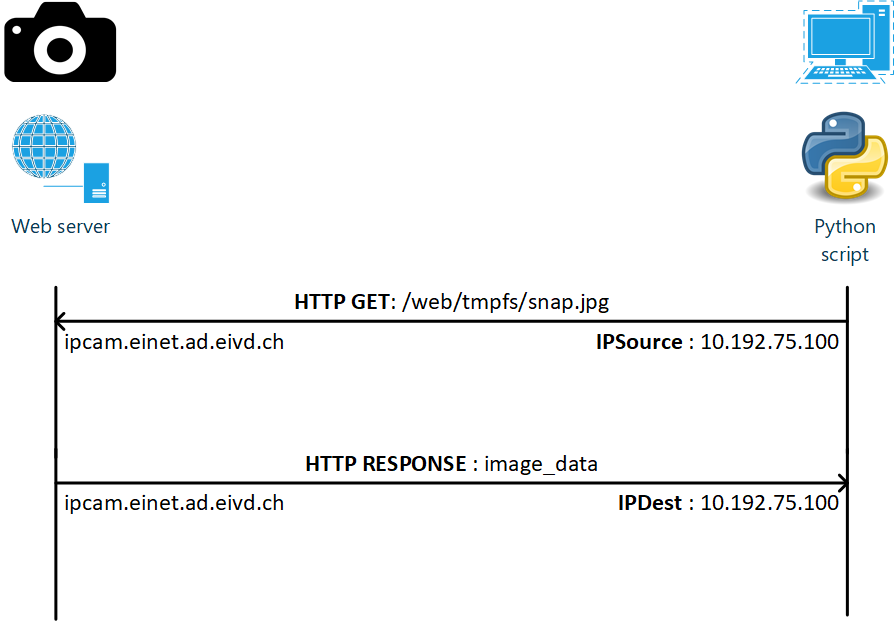
\includegraphics[width=130mm]{img/realisation/cam_request.png}
    \label{fig:image_request}
    \centering
    \caption{Requête d'une image à la caméra \textbf{Wanscam} \textit{HW0029-5}}
\end{figure} 

\subsection{Monitoring}
La caméra utilisée fonctionne sur batterie et panneaux solaires. Ainsi, il a semblé important de pouvoir surveiller le bon fonctionnement du système, et d'être averti en cas de malfonctions. On pensera notamment à une perte de connexion dûe à des batteries faibles (par exemple, suite à un manque de soleil sur plusieurs jours consécutifs), ou encore à un câble déconnecté.

\textit{Python} offre un système complet natif de journalisation. Lorsque ce système est utilisé dans les modules créés, il est aisé de traiter des \textit{logs}, et même d'avertir par mail des erreurs produites.

\todo{Logs}

\section{Traitement des images}
\subsection{Downsampling}
\subsection{Détection de bord}
\subsection{Evaluation des différentes méthodes et choix}
\subsection{Implémentation}
\begin{figure}[H]
    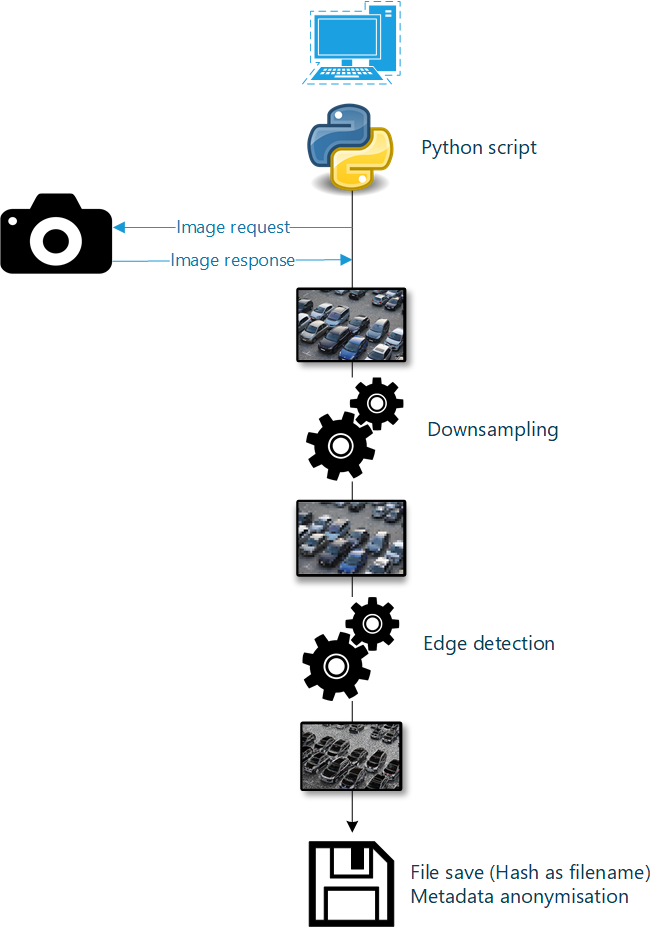
\includegraphics[width=130mm]{img/realisation/image_process.png}
    \label{fig:image_process}
    \centering
    \caption{Requêtes d'images et traitement}
\end{figure} 

\section{Annotations des images}

\section{Définition du réseau de neurone}

\section{Entrainement du modèle}



